\chapter{\IfLanguageName{dutch}{Stand van zaken}{State of the art}}%
\label{ch:stand-van-zaken}

% Tip: Begin elk hoofdstuk met een paragraaf inleiding die beschrijft hoe
% dit hoofdstuk past binnen het geheel van de bachelorproef. Geef in het
% bijzonder aan wat de link is met het vorige en volgende hoofdstuk.

% Pas na deze inleidende paragraaf komt de eerste sectiehoofding.
In dit hoofdstuk wordt de huidige stand van zaken rond de Cyber Resilience Act en geautomatiseerde CRA-compliance in een CI/CD-context besproken. Daarbij wordt eerst het wettelijk kader geschetst, om vervolgens in te gaan op bestaande praktijken en tools rond DevSecOps, security testing, SBOM-generatie en automatisch kwetsbaarheidsbeheer in pipelines. Het doel van dit hoofdstuk is enerzijds om voldoende theoretische en technische achtergrond te bieden zodat de lezer de uitwerking van de proof-of-concept in de volgende hoofdstukken goed kan situeren, en anderzijds om in kaart te brengen welke bestaande oplossingen hergebruikt kunnen worden en waar nog ontbrekende delen zijn waarvoor in deze bachelorproef zelf een oplossing moet worden uitgewerkt.

\section{Inleiding}

Er is de voorbije jaren een sterke evolutie geweest in onderzoek naar de automatisering van beveiligingstesten om gevaarlijke commits op te sporen en security-scans te integreren in het ontwikkelingsproces \autocite{Takahashi2025}. Omdat de complexiteit van software steeds toeneemt en supply-chain-aanvallen groeien, richten steeds meer bedrijven zich op DevSecOps, waarbij beveiliging vanaf het begin in de CI/CD-pipeline wordt geïntegreerd \autocite{Takahashi2025}. Met supply-chain-aanvallen worden aanvallen bedoeld waarbij niet de applicatie zelf rechtstreeks wordt aangevallen, maar zwakke schakels in de softwareketen, zoals externe dependencies, buildtools, repositories of updateprocessen \autocite{OWASPSupplyChain,LegitSupplyChain}. Ondertussen verplicht nieuwe Europese wetgeving, zoals de Cyber Resilience Act, fabrikanten van software- en hardwareproducten om hun producten duidelijk veilig en betrouwbaar te maken vóór deze op de markt komen \autocite{EU_CRA}. 

Deze literatuurstudie schetst de huidige stand van zaken rond CRA-compliance, beveiligingsautomatisering, SBOM-generatie en CVE-analyse, en toont welke problemen er vandaag nog bestaan.

\section{Cyber Resilience Act}
\subsection{Inleiding en doelstellingen}
De Cyber Resilience Act (CRA), die op 10 december 2024 in werking trad, is een Europese wetgeving die de cybersecurity van digitale producten verplicht stelt vóór deze op de markt komen \autocite{EU_CRA}. Het doel hiervan is het verbeteren van de digitale weerbaarheid van producten, met andere woorden: het vermogen van deze producten om veilig en betrouwbaar te blijven functioneren ondanks cyberdreigingen en het verkleinen van de risico's door kwetsbaarheden in software en hardware op tijd te detecteren en mitigeren. 

\subsection{Specifieke vereisten en tijdlijn}
De CRA legt strikte eisen op doorheen de volledige levenscyclus: security-by-design (risicoanalyse en secure development lifecycle), Software Bill of Materials (SBOM) voor transparantie van componenten, vulnerability management (CVE-scans en mitigatie), incidentrapportage binnen 24 uur bij ernstige kwetsbaarheden en verplichte beveiligingsupdates gedurende minstens 5 jaar \autocite{EU_CRA}. De implementatietijdslijn verloopt gefaseerd: meldplicht voor ernstige kwetsbaarheden start op 11 september 2026, volledige toepassing van alle eisen inclusief CE-certificering vanaf 11 december 2027 \autocite{RDI2024CRA}.
Figuur~\ref{fig:cra-tijdslijn} geeft een overzicht van enkele van de belangrijkste mijlpalen binnen de implementatietijdslijn van de Cyber Resilience Act.
\begin{figure}[h]
  \centering
  \begin{tikzpicture}[
      timeline/.style={-latex, thick},
      event/.style={circle, draw, fill=white, minimum size=8mm, inner sep=0pt},
      label/.style={align=center, font=\small}
  ]
    % As
    \draw[timeline] (0,0) -- (12,0);

    % 2024
    \node[event] (e2024) at (1.5,0) {};
    \node[label, above=8pt of e2024] {10 december 2024};
    \node[label, below=6pt of e2024] {CRA treedt\\in werking};

    % 2026
    \node[event] (e2026) at (6,0) {};
    \node[label, above=8pt of e2026] {11 september 2026};
    \node[label, below=6pt of e2026] {Start meldplicht\\kwetsbaarheden};

    % 2027
    \node[event] (e2027) at (10.5,0) {};
    \node[label, above=8pt of e2027] {11 december 2027};
    \node[label, below=6pt of e2027] {Volledige toepassing\\CRA-eisen};

    % Jaartallen wat hoger
    \node[font=\small] at (1.5,1.6)  {2024};
    \node[font=\small] at (6,1.6)    {2026};
    \node[font=\small] at (10.5,1.6) {2027};
  \end{tikzpicture}
  \caption{Implementatietijdslijn van de Cyber Resilience Act, op basis van de officiële CRA-tijdslijn\autocite{RDI2024CRA,EuropeanCommission2024CRAnews}.}
  \label{fig:cra-tijdslijn}
\end{figure}

\subsection{Impact voor bedrijven}
De nieuwe wetgeving zorgt voor zowel kansen als uitdagingen voor organisaties. Enerzijds stimuleert het innovatie en meer cyberveiligheid waardoor ook de betrouwbaarheid van de producten verhoogt, maar anderzijds bestaat er ook onduidelijkheid over specifieke productcategorieën, interpretatie van vereisten en implementatietijdlijnen van 36 maanden \autocite{ECSO2024}. Deze wetgeving is dan ook cruciaal voor bedrijven zoals Excentis, omdat naleving bepaalt of een product in aanmerking komt voor een CE-certificering \autocite{EuropeanCommission2024CRAnews}. Dit certificaat toont aan dat het product voldoet aan de CRA-wetgeving, wat zowel markttoegang als het vertrouwen van klanten en partners ondersteunt \autocite{RVO_CE}.

\subsection{CRA-Specifieke vereisten voor CI/CD}

De CRA verplicht geen gebruik van CI/CD-pipelines of automatisering, maar legt wel strikte cybersecurity-eisen op vóór marktintroductie. Deze moeten manueel of geautomatiseerd worden nageleefd, wat tijd, mankracht en dus kosten met zich meebrengt \autocite{Claranet2025}.

\section{CI/CD en DevSecOps}

\subsection{CI/CD fundamenten}
Continuous Integration (CI) en Continuous Delivery/Deployment (CD) is een manier om software sneller en betrouwbaarder te ontwikkelen. Dit staat voor de continue en automatische integratie van code door developers en het continue leveren en/of deployen van deze code door een operations team \autocite{RedHat2025}.

Er wordt binnen de CI/CD-omgeving steeds vaker DevSecOps toegepast, waarbij beveiliging vanaf het begin in de ontwikkelingscyclus wordt geïntegreerd \autocite{RamdassJain2025}. DevSecOps is een evolutie van de originele DevOps waar ook Security een centraal onderdeel wordt.

\subsection{DevSecOps principes}
DevSecOps rust op vijf kernprincipes die beveiliging integreren in de gehele softwareontwikkelingslevenscyclus \autocite{RamdassJain2025}:

\begin{itemize}
\item \textbf{Shift-left security}: Beveiliging wordt al geïmplementeerd in de vroegste ontwikkelfasen (IDE, eerste CI-stap) in plaats van pas aan het einde.
\item \textbf{Automatisering van security controls}: Alle securitytesten worden volledig geautomatiseerd in de CI/CD-pipeline (zie subsectie~\ref{subsec:security-testing-pipelines}).
\item \textbf{Policy-as-code}: Securityregels worden als code gedefinieerd en automatisch afgedwongen bij elke commit.
\item \textbf{Samenwerking Dev/Sec/Ops}: Ontwikkelaars, security en operations delen verantwoordelijkheid en werken met dezelfde tools.
\item \textbf{Continue monitoring}: Real-time dreigingsdetectie en vulnerability scanning blijven doorwerken na deployment.
\end{itemize}

Deze principes zorgen ervoor dat beveiliging geen bottleneck vormt maar een geïntegreerd onderdeel wordt van snelle softwareontwikkeling.

\subsection{Security testing in pipelines}\label{subsec:security-testing-pipelines}

In een DevSecOps-context worden verschillende soorten securitytesten geïntegreerd in de CI/CD-pipeline, zodat kwetsbaarheden zo vroeg mogelijk worden opgespoord \autocite{RamdassJain2025}. Daarbij wordt vaak een combinatie gebruikt van Static Application Security Testing (SAST), Dynamic Application Security Testing (DAST) en Software Composition Analysis (SCA), die automatisch draaien bij elke build of pull request \autocite{AWS2021}. Dit vermindert de kans dat kwetsbaarheden onopgemerkt in productie kunnen terechtkomen en helpt om sneller te reageren op nieuwe dreigingen \autocite{Snyk2026}.

Naast SAST, DAST en SCA worden in moderne DevSecOps-pipelines ook infrastructuurdefinities geanalyseerd via zogenaamde Infrastructure-as-Code (IaC)-scanners. Tools zoals Checkov voeren statische analyse uit op de Terraform-, Kubernetes- en andere IaC-bestanden op basis van een uitgebreide set beveiligings- en compliancepolicier \autocite{CheckovDoc,CheckovGithub}. Hiermee kunnen misconfiguraties, zoals publiek toegankelijke resources of ontbrekende encryptie, al vóór deployment worden opgespoord. Secrets-scanners analyseren broncode, configuratiebestanden en soms ook de volledige Git-historiek op patronen en hoge-entropy strings die op gelekte credentials wijzen \autocite{}. Trufflehog is een open source tool die zowel Git-repositories als filesystems kan scannen en daarbij ook verwijderde of niet meer zichtbare commits in de geschiedenis meeneemt, zodat gelekte secrets niet onbewust in producte kunnen terechtkomen \autocite{}

De OWASP Top 10 \autocite{OWASPTop10_2025} fungeert hierbij vaak als referentiekader om te bepalen welke soorten kwetsbaarheden minstens automatisch afgedekt moeten worden. Voor deze bachelorproef kan een shortlist van relevante categorieën worden opgesteld, zoals injectie, broken access control en kwetsbaarheden in afhankelijkheden, die door de pipeline automatisch getest worden. Tools zoals SAST-scanners voor broncode, DAST-scanners voor runtime-testing en dependency-scanners voor bibliotheken kunnen als aparte stappen in de pipeline worden geïntegreerd, waarbij de build wordt geblokkeerd als ernstige kwetsbaarheden worden gevonden.

\section{Software Bill of Materials}
\subsection{Wat is een Software Bill of Materials?}

Een Software Bill of Materials (SBOM) is een gestructureerde lijst van alle softwarecomponenten waaruit een applicatie of systeem is opgebouwd. Dit bevat typische velden zoals naam van de component, leverancier, versie, dependencies en metadata \autocite{IEEE2025}. Dit zorgt ervoor dat een organisatie beter zicht kan krijgen op hun software supply chain en sneller kwetsbaarheden en licentieproblemen kunnen identificeren \autocite{Stalnaker2024}.

SBOM-informatie wordt vastgelegd in gestandaardiseerde formaten zodat ze zowel door mensen als door tools verwerkt kan worden. De meest gebruikte hiervan zijn SPDX (Software Package Data Exchange) en CycloneDX \autocite{Stalnaker2024}. SPDX richt zich vooral op licenties, provenance en relaties tussen componenten en wordt onder andere aanbevolen in sectoren met strikte compliance eisen \autocite{Stalnaker2024}. CycloneDX is een lichter SBOM-formaat dat specifiek ontworpen is voor application security en supply-chain-risk-analyse, met ingebouwde ondersteuningen voor security- en kwetsbaarheidscontext \autocite{Stalnaker2024}.

\subsection{SBOM Generatie-tools}

SBOMs worden gegenereerd door tools die software dependencies analyseren tijdens de build-fase van CI/CD pipelines. \textcite{Mirakhorli2024} evalueerden 84 SBOM tools en identificeerden de tools met beste prestaties op basis van taal/ecosysteem ondersteuning.

\begin{table}[H]
  \centering
  \caption{Top SBOM Generatie-tools (Mirakhorli et al., 2024)}
  \begin{tabular}{|l|l|c|}
  \hline
  \textbf{Tool} & \textbf{Vendor} & \textbf{Talen/Ecosysteem} \\
  \hline
  CycloneDX Generator & CycloneDX & 14 \\
  Syft & Anchore & 14 \\
  Trivy & Aqua Security & 12 \\
  OSS Review Toolkit & ORT & 10 \\
  SPDX SBOM Generator & Independent & 9 \\
  \hline
  \end{tabular}
  \label{tab:sbom-tools}
\end{table}

Deze tools ondersteunen meerdere programmeertalen en package managers (Maven, npm, pip, etc.) en exporteren naar zowel SPDX als CycloneDX formaten \autocite{Mirakhorli2024}. 

Voor deze bachelorproef is \textbf{Syft} geselecteerd voor SBOM-generatie in de CI/CD pipeline. Deze keuze werd gemaakt op basis van verschillende criteria: het is een gratis en open source tool, het is in de voorgaande literatuur als één van de beste SBOM-generatietools voor containers beschouwd, en het integreert eenvoudig in Jenkins-pipelines. Syft kan daarbij niet alleen klassieke projectstructuren analyseren, maar ook containerimages, waardoor dezelfde tool zowel voor applicatie- als containergerichte SBOM-generatie kan worden ingezet \autocite{SyftGithub,AnchoreOpensource}.

\subsection{CRA-specifieke SBOM-vereisten}

De Cyber Resilience Act verplicht fabrikanten van producten met digitale elementen om een machine-leesbare SBOM te produceren, met minstens de top-level dependencies \autocite{EU_CRA}.

Dit moet dan ook voldoen aan volgende minimumeisen (BSI TR-03183-2):
\begin{table}[H]
  \centering
  \caption{BSI TR-03183-2: Vereiste SBOM data fields \autocite{BSI2025}}
  \begin{tabular}{|p{3cm}|p{8cm}|}
    \hline
    \textbf{Data field} & \textbf{Description} \\
    \hline
    Component creator & Email of URL van creator/maintainer \\
    Component name & Naam door creator toegewezen \\
    Component version & SemVer/CalVer of file modification date \\
    Filename & Exacte bestandsnaam (geen pad) \\
    Dependencies & Alle directe afhankelijkheden \\
    Distribution licences & Licentie(s) voor gebruik \\
    Hash value & SHA-512 van deployable component \\
    Executable property & executable/non-executable \\
    Archive property & archive/no archive \\
    Structured property & structured/unstructured \\
    \hline
  \end{tabular}
  \label{tab:cra-sbom-fields}
\end{table}
  
Hoewel BSI TR-03183-2 een Duitse richtlijn is, vormt deze de facto standaard voor heel de EU. Duitsland loopt voorop in CRA-implementatie en cybersecurity-wetgeving binnen Europa \autocite{Robyn2025}.

\section{CVE-Analyse en Vulnerability Management}
\subsection{NVD/CPE-matching}
CVE-Records worden verrijkt door de National Vulnerability Database (NVD) met gestructureerde metadata voor geautomatiseerde matching. De NVD bevat naast de CVE-details ook \textbf{CVSS-scores} (score van 0 tot 10, hoe hoger hoe ernstiger) en \textbf{CPE-matchcriteria} (gestandaardiseerde identifiers voor getroffen software/hardware) en referenties naar getroffen producten \autocite{NVD_API}.

CPE (Common Platform Enumeration) strings identificeren vendor, product en versie van getroffen software, volgens het gestandaardiseerde patroon van NIST \autocite{CPE_23}:
\begin{verbatim}
cpe:2.3:part:vendor:product:version:update:edition:lang:sw\_edition:
            target\_sw:target\_hw:other
\end{verbatim}

De matching-flow verloopt als volgt \autocite{NVD_API}:

%\begin{enumerate}
%    \item SBOM/dependency scan produceert lijst van componenten (naam en versie)
%    \item NVD CPE-criteria van CVE’s worden tegen componenten gematcht
%    \item Matches worden getoond met CVSS-score en exploit-details
%\end{enumerate}
\begin{figure}[h]
  \centering
  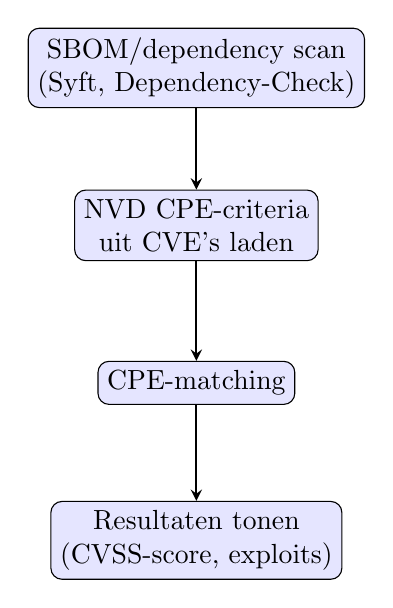
\begin{tikzpicture}[
      box/.style={rectangle, draw, rounded corners, minimum height=1.2em, minimum width=3em, align=center, fill=blue!10},
      arrow/.style={->, thick, >=stealth}
  ]
  
  % Nodes
  \node[box] (sbom) at (0,0) {SBOM/dependency scan\\(Syft, Dependency-Check)};
  \node[box] (nvd) at (0,-2) {NVD CPE-criteria\\uit CVE's laden};
  \node[box] (match) at (0,-4) {CPE-matching};
  \node[box] (result) at (0,-6) {Resultaten tonen\\(CVSS-score, exploits)};
  
  % Arrows
  \draw[arrow] (sbom) -- (nvd);
  \draw[arrow] (nvd) -- (match);
  \draw[arrow] (match) -- (result);
  
  \end{tikzpicture}
  \caption{Matching-flow SBOM naar CVE-detectie via NVD CPE-matching}
  \label{fig:cpe-matching-flow}
\end{figure}
Deze CPE-matching maakt geautomatiseerde vulnerability detection mogelijk in CI/CD pipelines.

\subsection{Dependency scanning tools}

Dependency scanning tools zijn tools die detectie van kwetsbare componenten in de software supply chains kunnen automatiseren door lockfiles en manifests te analyseren \autocite{Aikido2024}. Aangezien Jenkins het meest gebruikte CI/CD-platform is binnen de Excentis-omgevingen waar deze Proof of Concept wordt ontwikkeld, is er dan ook gekozen voor de \autocite{OWASPDependencyCheckPlugin} OWASP Dependency-check Jenkins plugin te gebruiken. Andere gekende open source voorbeelden hiervan zijn Dependabot (GitHub) en Snyk CLI, die beide de NVD-data en proprietary vulnerability databases combineren.

OWASP Dependency-Check scant alle populaire package managers (Maven, npm, pip, etc.) en genereert rapporten in HTML, XML en JSON formaten. De plugin integreert naadloos in Jenkins pipelines en kan builds laten falen bij kritieke vulnerabilities \autocite{OWASP2024}.

\subsubsection{Container image scanning}

Naast dependency-scanners op broncode bestaan er ook tools die specifiek containerimages analyseren op kwetsbaarheden. Deze tools combineren informatie overbesturingssysteempakketten en applicatie dependencies met gegevens uit kwetsbaarheidsdatabanken zoals de NVD \autocite{AnchoreOpensource,BionSyftGrype}.

Grype is een open source vulnerabilityscanner uit het Anchore-ecosysteem die containerimages, filesystems en SBOM-bestanden kan analyseren op bekende kwetsbaarheden \autocite{GrypeGithub}. De tool ondersteunt zowel rechtstreekse scans van images via Docekr of Podman als indirecte scans op basis van eerder gegenereerde SBOMs, bijvoorbeeld afkomstig van Syft \autocite{JitSyftGrype}. Dit zorgt er ook voor dat Grype makkelijk geïntegreerd kan worden in CI/CD-pipelines om containerimages nog vóór deployment automatisch te valideren op HIGH- en CRITICAL-kwetsbaarheden. 

\subsection{Risk scoring (CVSS)}

Het Common Vulnerability Scoring System (CVSS) is een open standaardkader om de ernst van kwetsbaarheden te kwantificeren op een schaal van 0.0 tot 10.0 \autocite{firstCVSSv4}. CVSS v4.0 (Common vulnerability Scoring System) toont de ernst aan van kwetsbaarheden op een schaal van 0.0 tot 10.0 via vier metriekgroepen: Base, Threat, Supplemental en Environmental \autocite{firstCVSSv4}

De \textbf{Base Score} berekent intrinsieke eigenschappen via 11 metrics:
\begin{itemize}
    \item \textbf{Exploitability}: Attack Vector (AV), Attack Requirements (AT), Privileges Required (PR), User Interaction (UI)
    \item \textbf{Impact}: Vulnerable System Confidentiality (VC), Integrity (VI), Availability (VA)
    \item \textbf{Attack Requirements (AT)}: nieuw in v4.0
\end{itemize}

\begin{table}[H]
  \centering
  \caption{CVSS v4.0 Base Score severity niveaus}
  \begin{tabular}{|l|c|}
  \hline
  \textbf{Score} & \textbf{Niveau} \\
  \hline
  0.0 & NONE \\
  0.1-3.9 & LOW \\
  4.0-6.9 & MEDIUM \\
  7.0-8.9 & HIGH \\
  9.0-10.0 & CRITICAL \\
  \hline
  \end{tabular}
  \label{tab:cvss-v4-scores}
\end{table}
  
In de Jenkins pipeline zal CVSS v4.0-scores gebruikt worden om builds te blokkeren bij HIGH/CRITICAL vulnerabilities (≥7.0).
\subsection{DAST-tools}

DAST-tools voeren dynamische security testing uit op runtime-applicaties, waarbij ze zich gedaragen als een externe aanvaller die probeert kwetsbaarheden te exploiteren. Verschillende studies evalueerden DAST-tools op basis van detectiecapaciteiten, false positive ratio en CI/CD-integratie \autocite{AIMultipleDAST2025,AppSecSanta2025}.

Tabel ~\ref{tab:dast-tools} toont een vergelijking van populaire DAST-tools op basis van open source licentie en Jenkins CI/CD-ondersteuning.

\begin{table}[H]
  \centering
  \caption{Top DAST-tools voor CI/CD integratie \autocite{AIMultipleDAST2025}}
  \begin{tabular}{|l|l|c|c|}
  \hline
  \textbf{Tool} & \textbf{Vendor} & \textbf{Open Source} & \textbf{Jenkins Support} \\
  \hline
  OWASP ZAP & OWASP & Ja & Ja \\
  Burp Suite & PortSwigger & Nee & Ja \\
  Acunetix & Invicti & Nee & Nee \\
  Netsparker & Invicti & Nee & Ja \\
  AppScan & HCL & Nee & Ja \\
  \hline
  \end{tabular}
  \label{tab:dast-tools}
\end{table}

OWASP ZAP springt eruit als de enige volledige open source oplossing met uitstekende CI/CD-ondersteuning via Docker en CLI. Het ondersteunt zowel passieve (header/cookie analyse) als actieve scanning (XSS, SQLi, CSRF) en genereert machine-leesbare rapporten voor quality gates \autocite{OWASPZAPDocs}.

Voor deze bachelorproef is \textbf{OWASP ZAP} geselecteerd als DAST-tool. De keuze werd gemaakt op basis van: open sourcel icentie, bewezen CI/CD-integratie via Docker/Jenkins, uitgebreide OWASP Top 10 dekking en gratis beschikbaarheid voor Excentis \autocite{OWASPZAPGithub}

\section{Toolselectie}

\subsection{Vergelijkende analyse van securitytools}

In deze bachelorproef is het doel om een DevSecOps-pipeline op te zetten die zowel kwetsbaarheden in eigen code alsook kwetsbaarheden in dependencies detecteert. Hiernaast moet dit ook een SBOM kunnen produceren die hergebruikt kan worden in functie van CRA-compliance. Dit betekent dat er tools nodig zijn die geïntegreerd kunnen worden in Jenkins zodat ze aansluiten bij de huidige ontwikkelpraktijk .

De selectie van deze tools vloeit voort uit de functionele eisen van de Proof of Concept: de pipeline moet code, dependencies, containers en secrets kunnen analyseren, SBOMs kunnen genereren en de resultaten integreren in Jenkins. Daarnaast wordt een vergelijking gemaakt met commerciële all-in-one platforms zoals Snyk en Aikido Security, om de gekozen open source aanpak te verantwoorden.

Daaril worden volgende tools besproken:
\begin{itemize}
  \item Snyk
  \item Aikido Security
  \item OWASP Dependency-Check
  \item SonarQube
  \item Grype
  \item Trufflehog
  \item Checkov
  \item OWASP ZAP
\end{itemize}

\subsubsection{Snyk}
Snyk positioneert zich als een developer-securityplatform dat verschillende soorten scantypes combineert \autocite{SnykFeatures}:
\begin{itemize}
  \item Snyk Code (SAST)
  \item Snyk Open Source (SCA)
  \item Snyk Container
  \item Snyk IaC
\end{itemize}

Dit platform ondersteunt zowel broncode- als dependency-analyse en kan integreren met bestaande SBOM-workflows voor kwetsbaarheidsanalyse en compliance-rapportering \autocite{SnykFeatures}. Snyk integreert met Jenkins via een officiële CLI en plugins, waardoor scans als aparte stages in de pipeline kunnen worden uitgevoerd \autocite{SnykJenkins}.

Voordelen in deze context:
\begin{itemize}
  \item Je hebt maar één platform nodig voor SAST, SCA, Container en IaC met uniforme rapportage.
  \item Standaardondersteuning voor de generatie van SBOM en koppeling aan NVD/CVE-data. 
  \item Het heeft goede integraties met Jenkins.
\end{itemize}

Nadelen:
\begin{itemize}
  \item Commerciële licentie is nodig voor volledige dekking (SAST, container, IaC) en valt dus buiten budget.
\end{itemize}
\subsubsection{Aikido Security}
Aikido biedt een geïntegreerd AppSecc-platform met zowel SAST als SCA-functionaliteit, gericht op lage false positives en eenvoudige integratie in bestaande DevOps-workflows \autocite{AikidoPlatform}.
Het platform combineert:
\begin{itemize}
  \item Statische code-analyse (SAST) voor eigen applicatiecode.
  \item Dependency scanning (SCA) voor open source libraries.
  \item Secrets scanning en IaC-analyse.
\end{itemize}
Aikido ondersteunt SBOM-achtige dependency-overzichten die gekoppeld worden aan vulnerability databases (zoals NVD). Voor Jenkins is er een "local scanner" die in de pipeline draait en resultaten terugstuurt naar het platform \autocite{AikidoJenkins}.

Voordelen in deze context:
\begin{itemize}
  \item Combineert SAST en SCA in één platform, met minder configuratie-inspanning dan aparte tools.
  \item Jenkins-integratie via local scanner, geschikt voor on-premises pipelines.
  \item Focus op lage false positive rates, wat ontwikkelaars minder frustreert en tijd bespaart, waardoor team moraal omhoog gaat.
\end{itemize}
Nadelen:
\begin{itemize}
  \item Commercieel platform met kosten voor volledige functionaliteit.
  \item Minder mature community en documentatie dan Snyk.
  \item SBOM-export functionaliteit is minder expliciet dan bij gespecialiseerde SCA-tools.
\end{itemize}

\subsubsection{OWASP Dependency-Check}

OWASP Dependency-Check is een Software Composition Analysis (SCA) tool en opensource plugin voor Jenkins die aan de hand van het OWASP framework de dependencies gaat bekijken en vergelijken met bekende kwetsbaarheden in de NVD-database \autocite{Jenkins2024}.

De tool analyseert:
\begin{itemize}
  \item Project manifests (Maven pom.xml, npm package.json, pip requirements.txt, etc.)
  \item Binary files en lockfiles voor component-identificatie
  \item Generatie van gedetailleerde rapporten (HTML, XML, JSON, CSV)
\end{itemize}
Dependency-Check gebruikt CPE-matching (zie Risk Scoring (CVSS)) om software en versies te koppelen aan CVE-records en CVSS v4.0-scores. Dit integreert perfect met Jenkins via een officiële plugin die scans uitvoert als pipeline-stage en builds kan blokkeren op basis van severity \autocite{Jenkins2024}.

Voordelen in deze context:
\begin{itemize}
  \item Volledig gratis en open source, perfect voor een bachelorproef
  \item Uitstekende Jenkins-integratie via officiële plugin
  \item Directe koppeling met NVD/CPE en CVSS-scoring uit vorige hoofdstukken
  \item Mature community en uitgebreide documentatie
\end{itemize}

Nadelen:
\begin{itemize}
  \item Alleen SCA-functionaliteit (geen SAST of DAST)
  \item Vereist aanvullende tools voor volledige code-analyse
  \item Kan false positives genereren bij complexe dependency-trees
\end{itemize}


\subsubsection{SonarQube}
SonarQube is een open source platform met een sterke focus op SAST (Static Application Security Testing) en codekwaliteitsmetrieken aan de hand van continue code-inspectie \autocite{SonarQubeFeatures}.

Het platform analyseert: 
\begin{itemize}
  \item Statische code-analyse (SAST) voor 30+ programmeertalen
  \item Security hotspots en kwetsbaarheden (SQL injection, XSS, etc.)
  \item Code smells, duplicatie en technische debt
  \item Quality gates voor CI/CD integratie
\end{itemize}

SonarQube biedt zowel een gratis (Community Edition) als een betalende (Enterprise add-on) aan. Voor geavanceerde SCA en SBOM-functionaliteit heb je de Enterprise add-on nodig. Dit integreert ook uitstekend met Jenkins via de officiële SonarScanner plugin \autocite{SonarJenkins}.

Voordelen in deze context:
\begin{itemize}
  \item Uitstekende SAST-functionaliteit voor eigen applicatiecode
  \item Gratis Community Edition voor bachelorproef
  \item Perfecte Jenkins-integratie met quality gates
  \item Grote community en uitgebreide documentatie
\end{itemize}

Nadelen:
\begin{itemize}
  \item Geen SCA of SBOM in gratis versie (alleen SAST)
  \item Advanced Security (SCA/SBOM) vereist betaalde Enterprise licentie
  \item Minder gericht op dependency-security dan gespecialiseerde SCA-tools
\end{itemize}

\subsubsection{Grype}

Grype is een open source vulnerabilityscanner die zich richt op containerimages en filesystems en deel uitmaakt van hetzelfde Anchore open source ecosysteem als Syft \autocite{AnchoreOpensource}.
De tool kan zowel rechtstreeks images scannen als SBOM-bestanden analyseren die eerder met Syft werden gegenereerd. Ook rapporteert Grype kwetsbaarheden met onder andere CVE-identifier, severity en CVSS-score \autocite{GrypeGithub,BionSyftGrype}.

Voordelen in deze context:
\begin{itemize}
  \item Gratis en open source.
  \item Sluit dicht aan op Syft: Syft genereert de SBOM, Grype gebruikt deze als input voor vulnerability-analyse.
  \item Eenvoudig te integreren in een Jenkins-pipeline via CLI-oproepen.
\end{itemize}

Nadelen:
\begin{itemize}
  \item Richt zich enkel op component- en image-level kwetsbaarheden (geen SAST of DAST).
  \item Net als andere scanners gevoelig voor false positives, zeker bij complexe images.
\end{itemize}

\subsubsection{Trufflehog (secrets-scanning)}

Trufflehog is een open source secrets-scanner die Git-repositoriesn Dockerimages en lokale filesystems analyseert op gelekte API-sleutels, tokens en andere gevoelige credentials \autocite{TrufflehogGithub,TrufflehogBlogGitVsFs}. De tool kan zowel de huidige toestand van de code als de volledige Git-historiek scannen en ondersteunt voor vele credentialtypes ook een vorm van verificatie, waarbij getest wordt of een gevonden secret nog actief is \autocite{TrufflehogDeepDive}. In de context van deze bachelorproef wordt Trufflehog gebruikt om te voorkomen dat hardcoded secrets aanwezig zijn wanner de CI/CD-pipeline wordt uitgevoerd.

\subsubsection{Checkov (IaC-scanning)}

Checkov is een open source static analysis-tool voor Infrastructure-as-Code die Terraform-, Kubernetes-, CloudFormation- en andere configuratiebestanden controleert op security- en complianceproblemen \autocite{CheckovDoc,CheckovGithub}. De tool gebruik policy-as-code regels om onder meer te detecteren of opslag niet versleuteld is, securitygroups te open zijn of cloudresources publiek toegankelijk zijn \autocite{CheckovTerraformGuide}. Hoewel Checkov relevant is voor een bredere DevSecOps-aanpak, valt dit in deze bachelorproef buiten de scope van de Proof of Concept.

\subsubsection{OWASP ZAP}
OWASP ZAP is een open source DAST-tool (Dynamic Application Security Testing) die runtime-scans uitvoert op actieve webapplicaties en API's. Het detecteert kwetsbaarheden zoals XSS, SQL-injectie, CSRF, broken access control en security misconfiguraties door zich te gedragen als een externe aanvaller \autocite{AppSecSanta2025,OWASPZAPDocs}.

De tool ondersteunt zowel passieve scanning (analyse van HTTP headers, cookies, etc.) als actieve scanning (geautomatiseerde exploit-pogingen) en genereert rapporten in HTML, JSON en XML formaat \autocite{OWASPZAPGithub}.
Voordelen in deze context:
\begin{itemize}
  \item Volledig gratis en open source (OWASP project).
  \item Uitstekende CI/CD-integratie via Docker containers en CLI-modus.
  \item Brede OWASP Top 10 dekking, inclusief moderne API-kwetsbaarheden.
  \item Actieve Jenkins plugin en community-ondersteuning.
\end{itemize}

Nadelen:
\begin{itemize}
  \item Vereist een draaiende applicatie (runtime testing, geen SAST).
  \item Kan false positives genereren bij complexe single-page applicaties (SPA's).
  \item Actieve scans duren langer dan statische analyse.
\end{itemize}
\begin{table}[h]
  \centering
  \caption{Vergelijking security tools voor Jenkins DevSecOps pipeline}
  \label{tab:tool-comparison}
  \begin{tabular}{|l|c|c|c|c|c|}
    \hline
    \textbf{Tool} & \textbf{SAST} & \textbf{SCA} & \textbf{SBOM} & \textbf{Jenkins} & \textbf{Licentie} \\
    \hline
    Snyk & Ja & Ja & Ja & Ja & Commercieel \\
    Aikido & Ja & Ja & Gedeeltelijk & Ja & Commercieel \\
    OWASP Dep-Check & Nee & Ja & Nee & Ja & Open Source \\
    SonarQube & Ja & Gedeeltelijk & Nee & Ja & Open Source* \\
    Grype & Nee & Ja (containers) & Ja (via SBOM) & Ja (CLI) & Open Source \\
    \hline
  \end{tabular}
  *Community editie gratis, Enterprise betaald
\end{table}




\subsubsection{Toolselectie}
Voor deze bachelorproef is gekozen voor de combinatie \textbf{Syft (SBOM), OWASP Dependency-Check (SCA op applicatieniveau), Grype (container image scanning)} en \textbf{SonarQube (SAST)}, omwille van:
\begin{itemize}
    \item \textbf{Volledig open source} (geen budgetbeperkingen)
    \item \textbf{Native Jenkins integratie}
    \item \textbf{Synergie}: SonarQube voor code-kwaliteit, Dependency-Check voor dependencies
\end{itemize}

\subsection{Bestaande CRA-compliance pipelines}

Hier zullen er twee concrete voorbeelden besproken worden van pipelines die voldoen aan CRA-vereisten zoals SBOM-generatie, CVE-scanning en compliance-rapportering. Deze cases tonen hoe de geanalyseerde tools in de praktijk worden ingezet.

\subsubsection{Red Hat Advanced Developer Suite (Enterprise Case)}

Red Hat's Advanced Developer Suite integreert SBOM-generatie, CVE-scanning en compliance-gating in een Jenkins-pipeline. De pipeline bevat:
\begin{enumerate}
  \item \textbf{SBOM-generatie}: Trusted Profile Analyzer produceert CycloneDX SBOMs
  \item \textbf{CVE-analyse}: SBOM wordt geüpload naar analyzer-service voor NVD-matching
  \item \textbf{Compliance-gate}: Builds falen bij kritieke vulnerabilities of policy-violaties
  \item \textbf{Audit-ready rapportage}: SBOMs en scan-resultaten worden gearchiveerd voor CRA-documentatie (zie Figuur~\ref{fig:redhat-pipeline})
\end{enumerate}


\begin{figure}[h]
  \centering
  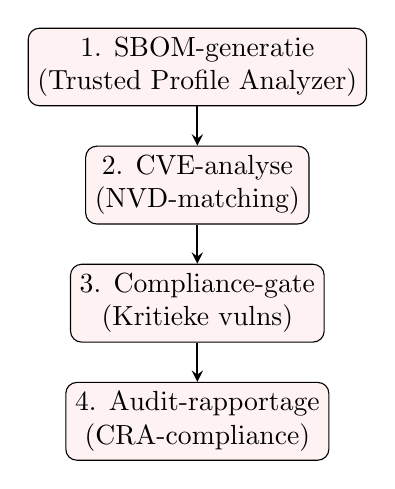
\begin{tikzpicture}[
      box/.style={rectangle, draw, rounded corners, minimum height=1.2em, minimum width=4em, align=center, fill=red!5},
      arrow/.style={->, thick, >=stealth}
  ]
  
  % Nodes (vertical flow)
  \node[box] (sbom) at (0,0) {1. SBOM-generatie\\(Trusted Profile Analyzer)};
  \node[box] (cve) at (0,-1.5) {2. CVE-analyse\\(NVD-matching)};
  \node[box] (gate) at (0,-3) {3. Compliance-gate\\(Kritieke vulns)};
  \node[box] (audit) at (0,-4.5) {4. Audit-rapportage\\(CRA-compliance)};
  
  % Arrows
  \draw[arrow] (sbom) -- (cve);
  \draw[arrow] (cve) -- (gate);
  \draw[arrow] (gate) -- (audit);
  
  \end{tikzpicture}
  \caption{Red Hat Advanced Developer Suite pipeline voor CRA-compliance}
  \label{fig:redhat-pipeline}
\end{figure}

Deze aanpak voldoet aan de vereisten van CRA door machine-readable SBOMs te maken alsook vulnerability-data te koppelen \autocite{RedHatPipeline}.

\subsubsection{Open Source Jenkins Pipeline (Syft + Trivy)}

Een open source template op GitHub toont een CRA-compliant pipeline met Syft voor SBOM en Trivy voor CVE-scanning \autocite{CRAEvidencePipeline}.

\begin{listing}[h]
  \caption{SBOM-generatie pipeline (Syft + archiveren)}
  \label{lst:pipeline-syft}
  \begin{minted}{groovy}
  pipeline {
    agent any
  
    stages {
      stage('Generate SBOM') {
        steps {
          sh '''
            curl -sSfL https://raw.githubusercontent.com/anchore/syft/main/install.sh | sh -s -- -b .
            ./syft dir:. -o cyclonedx-json > sbom.cdx.json
          '''
        }
      }
  
      stage('Archive SBOM') {
        steps {
          archiveArtifacts artifacts: 'sbom.cdx.json', fingerprint: true
        }
      }
    }
  }
  \end{minted}
\end{listing}

Deze pipeline produceert CycloneDX/SPDX SBOMs, scant voor CVEs en genereert audit-ready rapporten. Dit voldoet aan de BSI TR-03183-2 (de eisen voor de Duitse Overheid ivm. Cyber Resilience) en is direct bruikbaar voor Jenkins \autocite{CRAEvidencePipeline}. 

\section{Conclusie Literatuurstudie}

De literatuurstudie toont aan dat de bouwstenen voor het automatiseren van CRA-relevante securitycontroles in CI/CD-pipelines vandaag reeds in grote mate beschikbaar zijn. DevSecOps-praktijken, security testing in pipelines, SBOM-generatie en vulnerability management zijn technisch goed onderbouwd in de literatuur, en er bestaan zowel open source als commerciële tools die deze functionaliteiten ondersteunen. Voorbeelden hiervan zijn SonarQube voor statische codeanalyse (SAST), OWASP Dependency-Check voor dependency scanning (SCA), Syft voor SBOM-generatie, OWASP ZAP voor runtime web scanning (DAST) en Jenkins als CI/CD-pipeline voor integratie van deze controles.

Tegelijk maakt de literatuur ook duidelijk dat CRA-compliance niet kan worden herleid tot het louter combineren van enkele bestaande tools. Hoewel verschillende oplossingen deelaspecten van de problematiek afdekken, bestaat er nog geen eenduidige en gestandaardiseerde aanpak om CRA-vereisten technisch te vertalen naar concrete CI/CD-pipeline-stappen. Vooral op het vlak van toolintegratie, performantie-impact, false positives en de automatische validatie van CRA-specifieke compliancevereisten blijven er belangrijke uitdagingen bestaan.

Daarnaast blijkt dat commerciële platformen, zoals geïntegreerde enterprise-oplossingen, een aantal van deze problemen gedeeltelijk opvangen via gecentraliseerde workflows en uniforme rapportering, maar dat zulke oplossingen minder geschikt zijn binnen de context van deze bachelorproef wegens licentiekost, beperkte flexibiliteit en afhankelijkheid van vendor-specifieke ecosystemen.

Op basis van deze bevindingen is het daarom zinvol om in deze bachelorproef een eigen Proof of Concept uit te werken waarin open source componenten worden gecombineerd tot één werkende DevSecOps-pipeline. Deze PoC moet aantonen in welke mate CRA-relevante controles, zoals SBOM-generatie, dependency scanning en andere geautomatiseerde securitytesten, op een haalbare en reproduceerbare manier geïntegreerd kunnen worden binnen de ontwikkelcontext van Excentis.


%Deze literatuurstudie toont aan dat DevSecOps-praktijken en SBOM-generatie technisch goed gedocumenteerd zijn, met volwassen open source tools zoals OWASP Dependency-Check (SCA), SonarQube (SAST), Syft (SBOM) en Jenkins-integraties. Enterprise-oplossingen zoals Red Hat Advanced Developer Suite bieden geïntegreerde CRA-compliant workflows, maar vereisen commerciële licenties.

%\textbf{Bestaande oplossingen die direct gebruikt kunnen worden:}
%\begin{itemize}
%    \item \textbf{SCA}: OWASP Dependency-Check met NVD CPE-matching voor dependency-kwetsbaarheden
%    \item \textbf{SAST}: SonarQube Community Edition voor code-analyse  
%    \item \textbf{SBOM}: Syft/Trivy voor CycloneDX/SPDX generatie
%    \item \textbf{CI/CD}: Jenkins plugins voor pipeline-integratie
%\end{itemize}

%\textbf{Reikwijdte PoC-ontwikkeling:}
%\begin{itemize}
%    \item Tool-integratie en workflow-orkestratie in één consistente Jenkins pipeline
%    \item Performance-optimalisatie voor praktische ontwikkelworkflow
%    \item False positive filtering en baseline-mechanismen
%    \item CRA-specifieke compliance-validatie (nog ongestandaardiseerd)
%\end{itemize}

%De PoC zal deze bewezen componenten combineren tot een werkende, Excentis-specifieke DevSecOps pipeline die CRA-conformiteit automatiseert.




%\section{To be deleted}

%Dit hoofdstuk bevat je literatuurstudie. De inhoud gaat verder op de inleiding, maar zal het onderwerp van de bachelorproef *diepgaand* uitspitten. De bedoeling is dat de lezer na lezing van dit hoofdstuk helemaal op de hoogte is van de huidige stand van zaken (state-of-the-art) in het onderzoeksdomein. Iemand die niet vertrouwd is met het onderwerp, weet nu voldoende om de rest van het verhaal te kunnen volgen, zonder dat die er nog andere informatie moet over opzoeken \autocite{Pollefliet2011}.

%Je verwijst bij elke bewering die je doet, vakterm die je introduceert, enz.\ naar je bronnen. In \LaTeX{} kan dat met het commando \texttt{$\backslash${textcite\{\}}} of \texttt{$\backslash${autocite\{\}}}. Als argument van het commando geef je de ``sleutel'' van een ``record'' in een bibliografische databank in het Bib\LaTeX{}-formaat (een tekstbestand). Als je expliciet naar de auteur verwijst in de zin (narratieve referentie), gebruik je \texttt{$\backslash${}textcite\{\}}. Soms is de auteursnaam niet expliciet een onderdeel van de zin, dan gebruik je \texttt{$\backslash${}autocite\{\}} (referentie tussen haakjes). Dit gebruik je bv.~bij een citaat, of om in het bijschrift van een overgenomen afbeelding, broncode, tabel, enz. te verwijzen naar de bron. In de volgende paragraaf een voorbeeld van elk.

%\textcite{Knuth1998} schreef een van de standaardwerken over sorteer- en zoekalgoritmen. Experten zijn het erover eens dat cloud computing een interessante opportuniteit vormen, zowel voor gebruikers als voor dienstverleners op vlak van informatietechnologie~\autocite{Creeger2009}.

%Let er ook op: het \texttt{cite}-commando voor de punt, dus binnen de zin. Je verwijst meteen naar een bron in de eerste zin die erop gebaseerd is, dus niet pas op het einde van een paragraaf.

%\begin{figure}
%  \centering
%  \includegraphics[width=0.8\textwidth]{grail.jpg}
%  \caption[Voorbeeld figuur.]{\label{fig:grail}Voorbeeld van invoegen van een figuur. Zorg altijd voor een uitgebreid bijschrift dat de figuur volledig beschrijft zonder in de tekst te moeten gaan zoeken. Vergeet ook je bronvermelding niet!}
%\end{figure}

%\begin{listing}
%  \begin{minted}{python}
%    import pandas as pd
%    import seaborn as sns
%
%    penguins = sns.load_dataset('penguins')
%    sns.relplot(data=penguins, x="flipper_length_mm", y="bill_length_mm", hue="species")
%  \end{minted}
%  \caption[Voorbeeld codefragment]{Voorbeeld van het invoegen van een codefragment.}
%\end{listing}

%\begin{table}
%  \centering
%  \begin{tabular}{lcr}
%    \toprule
%    \textbf{Kolom 1} & \textbf{Kolom 2} & \textbf{Kolom 3} \\
%    $\alpha$         & $\beta$          & $\gamma$         \\
%    \midrule
%    A                & 10.230           & a                \\
%    B                & 45.678           & b                \\
%    C                & 99.987           & c                \\
%    \bottomrule
%  \end{tabular}
%  \caption[Voorbeeld tabel]{\label{tab:example}Voorbeeld van een tabel.}
%\end{table}

